% !TEX root = ../mainfile.tex
% !TEX encoding = UTF-8 Unicode
% !TEX spellcheck = en_US
%
% Chapter 6 — Structural VAR. Numbers generated by Code/06_var_analysis.py
% (recursive/Cholesky identification); verified against
% Output/tables/var_granger.csv, var_irf_dollar.csv, var_fevd_dollar.csv.

\chapter{Structural VAR Analysis}
\label{ch:svar}

The event study of Chapter~\ref{ch:event_study} identifies how the dollar responds to a
handful of \emph{discrete, dated} shocks. This chapter asks the complementary question:
over the full 2019--2026 sample, do continuous innovations to geopolitical risk, oil, and
risk sentiment transmit \emph{dynamically} to the dollar and the currency baskets day by
day? A recursively identified vector autoregression (VAR) answers it, and the answer
sharpens the event-study reading: the smooth geopolitical-risk index does \emph{not}
move the dollar at daily frequency---the safe-haven response is a feature of identifiable
events, not of the risk index in general.


\section{Specification and Diagnostics}
\label{sec:svar_diagnostics}

The system contains six daily variables, ordered from most to least exogenous: the change
in the Geopolitical Risk index ($\Delta\text{GPR}$), the Brent crude return, the change in
the VIX, the safe-currency basket return, the risky-currency basket return, and the broad
dollar return. The ordering encodes a standard recursive (Cholesky) identification:
geopolitical risk is treated as predetermined with respect to the financial variables
within the day, while the dollar---the most endogenous series---may react
contemporaneously to all of them but affects them only with a lag. All six series are
returns or first differences and are stationary: augmented Dickey--Fuller tests reject a
unit root at the $1\%$ level for every variable. The Akaike criterion selects four lags,
which the analysis adopts; the estimated system is stable (all companion-matrix
eigenvalues lie inside the unit circle). The sample is 1{,}941 trading days,
2019-01-03 to 2026-06-11.

Identification here is deliberately minimal. A recursive scheme is appropriate because the
question is directional---whether risk, oil, and sentiment shocks reach the dollar---rather
than a fully structural decomposition of simultaneous feedback. Robustness to the ordering
is discussed in Appendix~\ref{ch:appendix_a}.


\section{Granger Causality and Impulse Responses}
\label{sec:svar_irf_full}

Table~\ref{tab:var_granger} reports block Granger-causality tests. The result is clear and,
at first sight, surprising: \emph{the geopolitical-risk index does not Granger-cause the
dollar or either currency basket}---the $p$-values are $0.93$, $0.63$ and $0.37$. What does
move them is the VIX: a risk-sentiment shock Granger-causes the dollar ($p<0.001$), the
safe basket ($p<0.01$) and, more weakly, the risky basket. Oil innovations also feed the
dollar and the risky basket. Geopolitical risk, measured continuously, is not a daily
driver of exchange rates; risk sentiment and oil are.

\begin{table}[htbp]
\centering
\begin{threeparttable}
\caption{Granger causality: do the drivers predict the dollar and baskets?}
\label{tab:var_granger}
\small
\begin{tabular}{ll rr}
\toprule
Dependent & Driver & $F$ & $p$-value \\
\midrule
Broad USD     & $\Delta$GPR & $0.21$ & $0.934$ \\
Broad USD     & Brent       & $4.33$ & $0.002^{***}$ \\
Broad USD     & $\Delta$VIX & $8.38$ & $<0.001^{***}$ \\
\addlinespace
Safe basket   & $\Delta$GPR & $0.64$ & $0.633$ \\
Safe basket   & $\Delta$VIX & $4.17$ & $0.002^{***}$ \\
\addlinespace
Risky basket  & $\Delta$GPR & $1.07$ & $0.371$ \\
Risky basket  & Brent       & $6.07$ & $<0.001^{***}$ \\
Risky basket  & $\Delta$VIX & $2.10$ & $0.078^{*}$ \\
\bottomrule
\end{tabular}
\begin{tablenotes}[flushleft]\footnotesize
\item \textit{Notes.} Block $F$-tests from the six-variable daily VAR(4), 2019--2026.
$^{*}/^{**}/^{***}$: 10/5/1\%.
\end{tablenotes}
\end{threeparttable}
\end{table}

The orthogonalised impulse responses in Figure~\ref{fig:var_irf} make the same point
visually. A one-standard-deviation geopolitical-risk shock leaves the broad dollar
essentially unmoved: the cumulative response after fifteen trading days is $+0.01\%$, with
the $90\%$ band straddling zero. A VIX shock, by contrast, appreciates the dollar by a
significant $+0.15\%$---the safe-haven reflex, now identified from the continuous series
rather than from a single event---while an oil shock nudges it down by a small but
significant $-0.08\%$.

\begin{figure}[htbp]
  \centering
  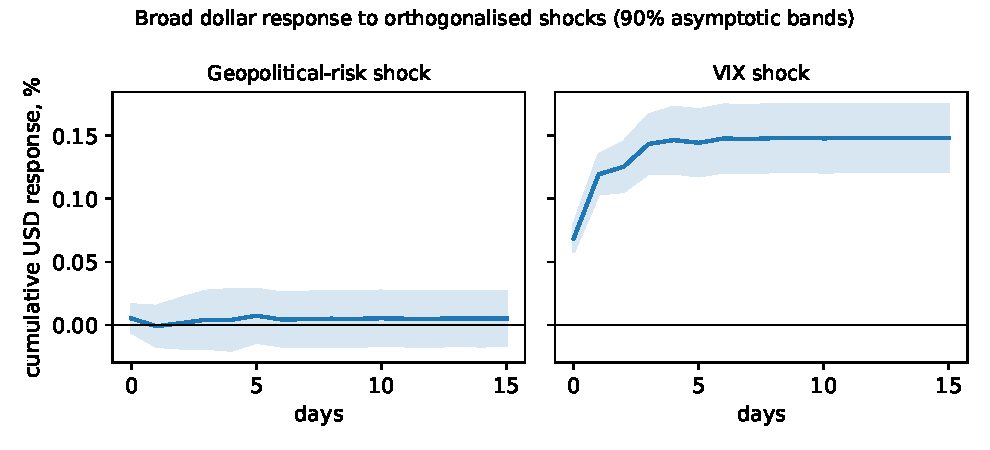
\includegraphics[width=\linewidth]{var_irf_gpr}
  \caption[Dollar impulse responses to risk and sentiment shocks]{Cumulative response of
  the broad dollar index to orthogonalised shocks, with $90\%$ asymptotic bands. The dollar
  does not respond to a geopolitical-risk shock (left) but appreciates significantly after a
  VIX shock (right).}
  \label{fig:var_irf}
\end{figure}


\section{Forecast Error Variance Decomposition}
\label{sec:svar_fevd}

The variance decomposition confirms the magnitudes. At a ten-day horizon, geopolitical-risk
shocks account for $0.1\%$ of the broad dollar's forecast-error variance, oil for $1.8\%$,
and the VIX for $7.9\%$; the remainder is the dollar's own innovations and the currency
baskets (Table~\ref{tab:var_fevd}). Whatever the geopolitical-risk index contributes to the
dollar, it does so not through a measurable daily linear channel but through the discrete,
high-salience events isolated in Chapter~\ref{ch:event_study}.

\begin{table}[htbp]
\centering
\begin{threeparttable}
\caption{Forecast error variance decomposition of the broad dollar (\%)}
\label{tab:var_fevd}
\small
\begin{tabular}{l rrrrrr}
\toprule
Horizon & $\Delta$GPR & Brent & $\Delta$VIX & Safe & Risky & USD own \\
\midrule
$h{=}1$  & $0.1$ & $1.1$ & $7.6$ & $49.9$ & $6.4$ & $34.9$ \\
$h{=}5$  & $0.1$ & $1.8$ & $7.9$ & $49.2$ & $6.4$ & $34.7$ \\
$h{=}10$ & $0.1$ & $1.8$ & $7.9$ & $49.2$ & $6.4$ & $34.7$ \\
\bottomrule
\end{tabular}
\begin{tablenotes}[flushleft]\footnotesize
\item \textit{Notes.} Share of the broad dollar's forecast-error variance attributable to
each orthogonalised shock, recursive ordering as in Section~\ref{sec:svar_diagnostics}.
\end{tablenotes}
\end{threeparttable}
\end{table}


\section{Interpretation and Caveats}
\label{sec:svar_subsample}

The VAR and the event study are two readings of the same object that agree once the
distinction between a \emph{level} and an \emph{event} is taken seriously. Geopolitical risk
moves the dollar when it arrives as a discrete, interpretable shock---an invasion, a tariff
announcement, a strait closure---whose direction the market can price; the running GPR
index, which also rises on diffuse, ambiguous news, carries no such daily signal and so
predicts nothing. Risk sentiment (the VIX) is the channel through which acute episodes reach
the dollar, which is why the safe-haven reflex shows up in the VIX impulse response.

Three caveats bound these results. First, identification rests on the recursive ordering;
plausible reorderings are examined in Appendix~\ref{ch:appendix_a} and leave the
qualitative picture unchanged. Second, a formal split into a tariff subsample and an Iran
subsample is not pursued: each window is too short for a stable six-variable VAR, and the
event study already provides the cleaner episode-by-episode identification. Third, the daily
GPR index is itself a noisy text-based measure, which biases its estimated daily effect
toward zero---a reason to read the null as ``no measurable linear daily channel'' rather
than ``no role for geopolitics,'' a role the event study documents directly.
